% !TEX encoding = UTF-8
% !TEX TS-program = pdflatex
% !TEX root = ../tesi.tex

%**************************************************************
\chapter{Descrizione dello stage}
\label{cap:descrizione-stage}
%**************************************************************

\intro{In questo capitolo si introduce il contesto in cui lo stage viene svolto e viene fornita una panoramica del progetto. Successivamente si descrivono le principali tecnologie utilizzate per raggiungere gli obiettivi prefissati. Inoltre sono analizzati i vincoli, gli obiettivi e la pianificazione dello stage.}\\

%**************************************************************
\section{Introduzione al progetto}
\subsection{L'idea}
L’obiettivo di Sync Lab è sviluppare un’applicazione per il \emph{\gls{contact tracing}}\glsfirstoccur.
Il software deve poter registrare i contatti tra le persone sfruttando il \emph{\gls{bluetooth LE}}\glsfirstoccur. Le informazioni da raccogliere riguardano il tempo e la distanza di contatto con gli altri dispositivi, assicurando il rispetto della privacy. Quando una persona risulta infetta deve essere data la possibilità di inserire il suo stato nel sistema e di avvisare chi è entrato in contatto con questa persona tramite notifica del telefono.\\

L’azienda ha incaricato diversi stagisti di sviluppare un’applicazione mobile e una web application che gestiscano il \textit{contact tracing}, la prima lato utente generico, la seconda per il personale sanitario. 
Lo scopo dell'applicazione mobile è quello di registrare i contatti, mentre lo scopo della web app è fornire l’autorità al personale medico di segnalare una persona risultata positiva a un tampone, sempre dietro conferma del malato.\\

Questo è il quadro generico dove si inserisce il mio percorso di stage.
Mi è stato proposto di studiare e implementare uno \textit{smart contract} per registrare i contatti nella piattaforma \emph{\gls{Ethereum}}. 
I punti principali da affrontare durante il periodo del mio stage sono i seguenti:
\begin{itemize}
	\item{Studio tecnologico delle \textit{blockchain} (in particolare \textit{Ethereum});}
	\item{Analisi e sviluppo di uno \textit{smart contract} per il \textit{contact tracing} in linguaggio \textit{Solidity};}
	\item{Studio e utilizzo dello smart contract in ambiente mobile (Android).}
\end{itemize}

\subsection{Motivazioni}
La pandemia di Covid-19 ha messo alla luce il bisogno di utilizzare applicazioni mobile per il \textit{contact tracing}, in modo da prevenire la diffusione della malattia.  
Le motivazioni dell'azienda per sviluppare SyncTrace, dunque, appaiono abbastanza chiare. La domanda che sorge più spontanea riguarda l'utilizzo della \textit{blockchain} per questo scopo.\\\\
Il contact tracing può portare a problemi di privacy perché richiede che le informazioni siano conservate e distribuite tra i dispositivi; inoltre è necessario garantire la protezione dell'identità degli utenti infetti. La blockchain può giocare un ruolo neutrale nella trasmissione di questi dati sensibili, fornendo una soluzione per la privacy grazie alla sua natura che garantisce immutabilità, incorruttibilità, anonimato e sicurezza.\\
Per esempio, nelle soluzioni più utilizzate per il contact tracing, è possibile attaccare il sistema per corrompere le informazioni. Un \textit{replay attack} non è da escludere: un attaccante potrebbe impossessarsi delle credenziali di un dispositivo per simulare contatti inesistenti; utilizzando la blockchain si scongiurano questo tipo di pericoli.


%**************************************************************

\section{Studio tecnologico}
Lo studio richiesto per lo svolgimento dello stage parte dalla tecnologia \textit{blockchain} in tutti i suoi aspetti, per poi passare allo studio specifico di \textit{Ethereum}, \textit{Solidity} e tutti gli strumenti di supporto per lo sviluppo e il testing di \textit{smart contract}. Infine è necessario capire come integrare lo \textit{smart contract} sviluppato in un ambiente mobile e in una web application.

\subsection{Blockchain}
Una \textit{blockchain} è un registro pubblico e decentralizzato che offre la possibiltà di avere un database distribuito contenente tutte le transazioni eseguite e condivise tra i partecipanti della rete. Questo database viene chiamato \emph{\gls{distributed ledger}}\glsfirstoccur, in italiano libro mastro decentralizzato.
Tutte le transazioni realizzate vengono conservate nel \textit{ledger}, che è pubblico, sicuro e immutabile. Ogni transazione nel \textit{ledger} pubblico è verificata dalla maggioranza dei partecipanti grazie a un \emph{\gls{algoritmo di consenso}}\glsfirstoccur.\\\\ Le principali caratteristiche delle \textit{blockchain} sono:
\begin{itemize}
	\item{\textbf{Immutabilità: } quando una transazione è accettata e validata non può più essere cancellata o modificata;}
	\item{\textbf{Decentralizzazione: }la rete è distribuita sui nodi di tutti i partecipanti, permettendo diversi vantaggi come l'assenza di un \emph{single point of failure}\glsfirstoccur;}
	\item{\textbf{Anonimato: }è garantito l'anonimato dell'identità degli utenti che effettuano una transazione;}
	\item{\textbf{Sicurezza: }grazie all'assenza di un \textit{single point of failure} la sicurezza di una \textit{blockchain} è superiore rispetto a un tradizionale database centralizzato;}
	\item{\textbf{Capacità: }avere a disposizione un gran numero di macchine che lavorano inseme come un'unica entità si traduce in una grande potenza di calcolo e di capacità del database.}
\end{itemize}

\subsubsection{Permissionless e permissioned}
Le blockchain si dividono in due categorie: \textit{blockchain} \emph{\gls{permissionless}}\glsfirstoccur (o pubbliche) e \textit{blockchain} \emph{\gls{permissioned}}\glsfirstoccur (o private). Le prime permettono a qualsiasi utente che decida di connettersi, di generare nuove transazioni, effettuare il compito di \emph{\gls{miner}}\glsfirstoccur o leggere il registro delle transazioni memorizzate. \emph{\gls{Bitcoin}}\glsfirstoccur ed \textit{Ethereum}\glsfirstoccur sono esempi di \textit{blockchain} pubbliche.
Le seconde, invece, permettono l’accesso solo ad utenti autorizzati e autenticati, poiché la \textit{blockchain} opera esclusivamente entro i limiti di una comunità ben definita dove tutti i partecipanti sono noti. Solitamente a capo di questi sistemi si trovano istituti finanziari o agenzie governative che definiscono chi possa accedere o meno alla rete. Nelle \textit{blockchain permissioned}, tutti i \textit{miner} sono considerati fidati.

\subsubsection{Nodi, transazioni, blocchi, ledger}
Per comprendere al meglio il funzionamento di una \textit{blockchain} è utile spiegare i componenti basilari da cui è formata:
\begin{itemize}
	\item{\textbf{Nodi: }sono i partecipanti alla \textit{blockchain}. Qualsiasi dispositivo che si connette alla blockchain è considerato un nodo; ne esistono di diversi tipi in base al ruolo che hanno nella rete;} 
	\item{\textbf{Transazioni: }sono le azioni generate dai partecipanti al sistema, costituite dai dati scambiati. Necessitano di essere verificate, approvate e poi archiviate;}
	\item{\textbf{Blocchi: }sono un raggruppamento di transazioni validate che vengono registrate nella \textit{blockchain}, assicurando la corretta sequenza e la certezza che le informazioni registrate non siano state manomesse;}
	\item{\textbf{Distributed ledger: } è il registro pubblico nel quale vengono annotate con la massima trasparenza e in modo immutabile tutte le transazioni effettuate in modo ordinato e sequenziale. Il \textit{ledger} è costituito dall’insieme dei blocchi che sono tra loro incatenati tramite una funzione di crittografia, grazie all’uso di \emph{\gls{hash}}\glsfirstoccur.}
\end{itemize}

\subsubsection{Generali bizantini}
La \textit{blockchain} nasce per eliminare il bisogno di una terza parte che validi una transazione. Per farlo è necessario che tutti i nodi siano concordi sulla validità e l’ordine delle transazioni. È dunque fondamentale introdurre un algoritmo di consenso per approvare i blocchi e quindi le transazioni. Per capire appieno questo concetto è ragionevole introdurre il problema matematico dei generali bizantini.\\\\
Diversi generali, durante un assedio, sono sul punto di attaccare una città nemica. Essi sono dislocati in diverse aree strategiche e possono comunicare solo mediante messaggeri al fine di coordinare l’attacco decisivo.
Il problema è che tutti sanno che tra di loro si trovano uno o più traditori. 
Come può ciascun luogotenente avere la certezza che, una volta ricevuto l’ordine di attacco, questo sia stato inviato anche agli altri? Come può essere certo di non essere l’unico ad averlo ricevuto in quella forma e dunque che tutti gli altri luogotenenti siano nella condizione di trasmettere e condividere lo stesso ordine?
Come è possibile garantire ai generali e a tutti i luogotenenti che nessuno cerchi di minare il piano?
\begin{figure}[h]
\caption{Problema dei generali bizantini}
\centering
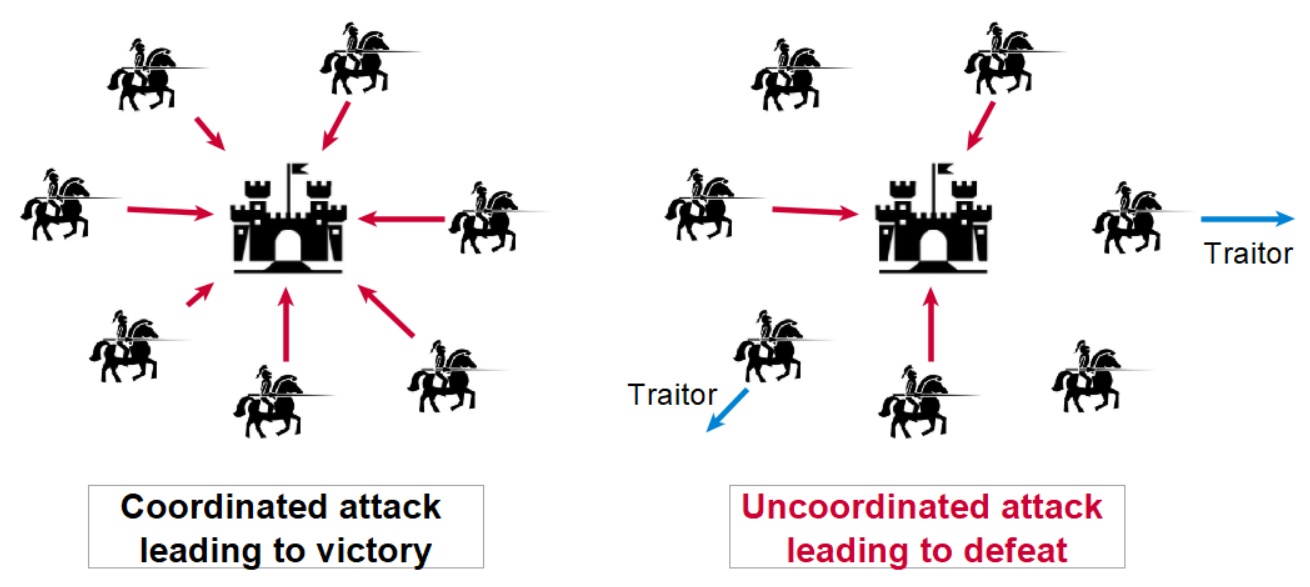
\includegraphics[width=1.0\textwidth]{./immagini/bizantini}
\end{figure}

L'obiettivo da raggiungere è far sì che ai luogotenenti onesti arrivi il piano d’attacco corretto, senza che i traditori possano compromettere l’operazione facendo arrivare loro le informazioni sbagliate.
In una \textit{blockchain}, la soluzione è quella di non avere più un generale che comanda sugli altri. Non c’è più un centro che prevale gerarchicamente, ma si assegna la stessa gerarchia a tutti i partecipanti. Tutti i generali e tutti i luogotenenti, ovvero tutti i nodi, che partecipano a questo modello, concordano ogni singolo messaggio trasmesso, lo vedono e lo condividono. Di conseguenza la \textit{blockchain} è incorruttibile se la maggioranza dei partecipanti risulta essere onesta.


\subsubsection{Algoritmi di consenso}
Gli algoritmi di consenso assicurano la sicurezza e l'integrità dei dati nei sistemi distribuiti. In una \textit{blockchain} l'obiettivo di questi algoritmi è ottenere la validazione delle transazioni, rendere la rete affidabile e prevenire gli attacchi da parte di malintenzionati.
Per ottenere questo risultato i nodi partecipanti devono essere d'accordo sullo stato della \textit{blockchain}. Ogni transazione deve essere registrata nel \textit{ledger} e l’algoritmo di consenso assicura che non ci siano state transazioni maligne o corrotte.
Esistono diversi tipi di algoritmi, ma mi limiterò a spiegare i due principali, su cui si fonda la quasi totalità delle \textit{blockchain}.\\

\paragraph{Proof of work}
L’algoritmo \emph{\gls{proof of work}}\glsfirstoccur si basa sulla generazione di blocchi attraverso complessi problemi matematici, la cui risoluzione richiede un grande sforzo computazionale.
Il meccanismo su cui si basa questo algoritmo è la ricerca di un valore che sottoposto a una funzione \textit{hash} risulti iniziare con un certo numero di zeri. Il lavoro medio è esponenzialmente proporzionale al numero di zeri richiesti. Quello che rende adatto l'\textit{hash} per questo genere di algoritmo è il fatto che sia molto difficile trovare un valore che corrisponda alle caratteristiche richieste, ma estremamente facile verificarne la correttezza.\\ 
Generalmente si adotta un valore \textit{hash} con un numero selezionabile di prime cifre a zero. Il nodo che riesce a trovare il valore \textit{hash} corretto prima degli altri crea il blocco: esso verrà aggiunto in coda alla \textit{blockchain} e riceverà un compenso sotto forma di valuta virtuale, chiamata \emph{\gls{criptovaluta}}\glsfirstoccur.\\ L’algoritmo \textit{proof of work} risolve il problema dei generali bizantini se almeno il 50\% + 1 dei partecipanti alla \textit{blockchain} è onesta: soffre infatti dell'attacco del 51\%.  Se la maggioranza della potenza computazionale della rete fosse controllata da un attaccante o un gruppo di attaccanti, questi avrebbero la possibilità di escludere intenzionalmente transazioni o modificarle a proprio piacimento. Un attacco di questo tipo consentirebbe all'attaccante di invertire le transazioni che ha effettuato, portando a un \emph{\gls{double spending}}\glsfirstoccur. Questo scenario potrebbe fare pensare a gravi problemi di sicurezza nelle \textit{blockchain}, ma in realtà subire un attacco di questo tipo è altamente improbabile, soprattutto nelle \textit{blockchain} di ampia diffusione. Quando una \textit{blockchain} diventa sufficientemente grande, la possibilità che una singola persona o un singolo gruppo di persone sia in grado di controllare il 51\% della rete è quasi nulla.

\paragraph{Proof of stake}
Nel \textit{proof of stake} i blocchi vengono validati da chi possiede più \emph{\gls{token}}\glsfirstoccur nella \textit{blockchain}. Ogni account ha una possibilità proporzionale al proprio saldo di generare un blocco valido. Rispetto al \textit{proof of work}, questo approccio presenta molti vantaggi. Il \textit{proof of work} richiede un'enorme quantità di tempo ed energia e, di conseguenza, un limitato numero di transazioni al secondo e un costo elevato da parte dell’utente per ottenere la validazione della propria transazione. Con il \textit{proof of stake} si ottiene maggiore scalabilità e minor costo per le transazioni.
Inoltre la struttura della \textit{blockchain} la rende più sicura. Se un \textit{miner} detiene la maggioranza dello \textit{stake}, non ha nel suo interesse un attacco alla rete perché se il valore della criptovaluta crolla, crollerebbero anche tutti i suoi averi. Per questo i maggiori proprietari di token hanno nel loro interesse il mantenimento di una rete sicura.

Il \textit{proof of work} è stato il primo algoritmo utilizzato nelle \textit{blockchain} ed è tutt’ora il più diffuso. Negli ultimi anni però stanno nascendo molte \textit{blockchain} che si basano su \textit{proof of stake} e persino \textit{Ethereum}, entro la fine del 2020, inizierà il passaggio al \textit{proof of stake}, che si dovrebbe completare nel 2022.

\subsection{Ethereum}
\textit{Ethereum} è una piattaforma \textit{blockchain} creata nel 2015 da Vitalik Buterik e che ha riscosso fin da subito grande successo.  È nata come alternativa a \textit{Bitcoin}, proponendo la possibilità di eseguire programmi chiamati \textit{smart contract} per creare applicazioni decentralizzate. Anche \textit{Bitcoin} ha un linguaggio che gli permette di creare \textit{smart contract}, ma a differenza della famosa \textit{blockchain}, in \textit{Ethereum} è possibile scrivere contratti \emph{\gls{turing completi}}\glsfirstoccur. Negli \textit{smart contract} è possibile programmare come in qualsiasi altro linguaggio di programmazione, seppur con delle differenze di cui discuteremo più avanti. 


\subsubsection{Smart contract}
Un contratto è un insieme di codice e dati che si trova a uno specifico \textit{address} di \textit{Ethereum}. È un vero e proprio programma che viene eseguito dai nodi della \textit{blockchain}. Gli \textit{smart contract} possono leggere o modificare il proprio stato interno, oltre a mandare o ricevere messaggi e transazioni. Esistono diversi linguaggi che permettono lo sviluppo di \textit{smart contract} in \textit{Ethereum}. I più famosi sono:
\begin{itemize}
	\item{\textit{Solidity}, simile a \textit{JavaScript};}
	\item{\textit{Vyper}: simile a \textit{Python}.}
\end{itemize}
\textit{Solidity} è sicuramente il più diffuso per lo sviluppo di \emph{\gls{applicazioni decentralizzate}}\glsfirstoccur e, per questo motivo, è stato utilizzato durante lo stage.

\subsubsection{Account, transazioni e gas}
\paragraph{Account}\mbox{}\\
In Ethereum ogni partecipante alla blockchain possiede un account con cui interagire nella rete. Anche gli smart contracts hanno un account, fondamentale per raggiungerli e interagire con loro. Gli account hanno un \textit{balance} in \emph{\gls{Ether}}\glsfirstoccur che può essere modificato da transazioni inviate o ricevute.
\paragraph{Transazioni}\mbox{}\\
Una transazione è composta dall'\textit{account target}, l'\textit{account sender}, il valore trasferito in \textit{Ether}, campi dati opzionali, il limite di gas che la transazione può consumare e il prezzo del gas.
\paragraph{Gas}\mbox{}\\
Le transazioni consumano un certo numero di gas, che rappresenta il carburante della blockchain. Ogni operazione negli smart contract ha un costo in gas, detto \emph{\gls{gas price}}\glsfirstoccur, con cui viene calcolato il prezzo della \emph{\gls{fee}}\glsfirstoccur da pagare ai \textit{miner} in \textit{Ether}. Inoltre le operazioni hanno anche un limite di gas, detto \emph{\gls{gas limit}}\glsfirstoccur, ossia la massima quantità di gas che può essere consumata in una transazione. Questo limite protegge la \textit{blockchain} dai \textit{loop} infiniti.

\begin{figure}[!htb]
   \begin{minipage}{0.48\textwidth}
     \centering
     
\includegraphics[width=0.4\textwidth]{./immagini/logo_ethereum}
     \caption{Logo di Ethereum}
   \end{minipage}\hfill
   \begin{minipage}{0.48\textwidth}
     \centering
     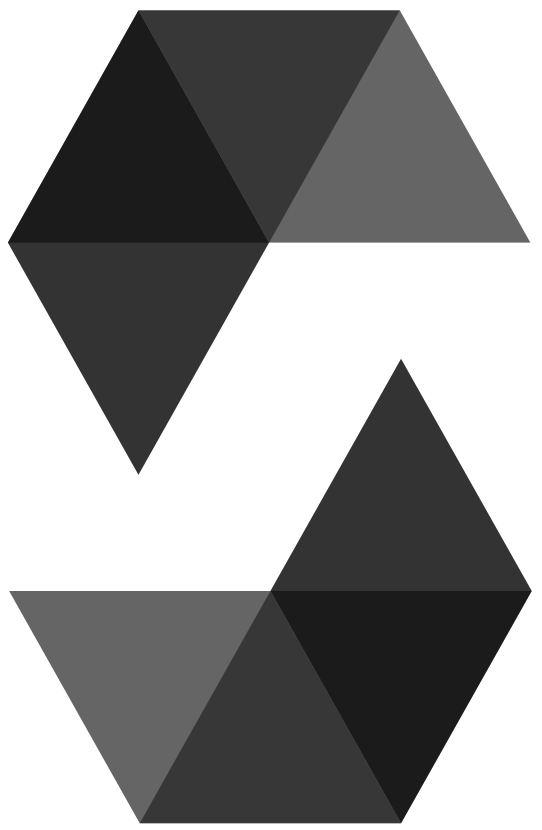
\includegraphics[width=0.425\textwidth]{./immagini/logo_solidity}
     \caption{Logo di Solidity}
   \end{minipage}
\end{figure}

\subsubsection{Solidity}
\textit{Solidity} è un linguaggio tipato che permette di scrivere \textit{smart contract}. I \textit{contratti} a prima vista ricordano molto le classi nella programmazione orientata a oggetti. In \textit{Solidity}, però, bisogna prestare particolare attenzione alla sicurezza, in quanto gli \textit{smart contract} si occupano di gestire transazioni. Se sono presenti bug o falle di sicurezza le conseguenze potrebbero essere gravi. Inoltre è sempre opportuno tenere a mente che le operazioni non sono gratuite, ma vengono pagate con delle \textit{fee} in base al tipo di operazione richiesta. L'efficienza quindi, è cruciale nel definire \textit{smart contract} e non sempre le \emph{\gls{best practices}}\glsfirstoccur in \textit{Solidity} corrispondono alla soluzione che può sembrare migliore in un altro linguaggio di programmazione.

\newpage
Di seguito viene riportato un contratto a titolo esemplificativo:
\begin{lstlisting}[language = Solidity]
pragma solidity ^0.6.8;

contract HelloWorld {

	string hello;
	
	constructor() public {
	    hello = "Hello World!";
	}

	function getHello() public view returns (string memory) {
		return hello;
	}

	function setHello(string memory _hello) public {
		hello = _hello;
	}
}

\end{lstlisting}

\subsubsection{Truffle}
\textit{Truffle} è una suite di supporto per la programmazione in \textit{Solidity} che ha l'obiettivo di rendere la vita dello sviluppatore più semplice. Fornisce un ambiente di sviluppo e un \textit{framework} per testare i contratti usando una \textit{EVM} (\emph{\gls{Ethereum Virtual Machine}}\glsfirstoccur). 
\subsubsection{Web3js e web3j}
Tra gli obiettivi del mio stage c'è l'integrazione dello \textit{smart contract} sviluppato con un ambiente mobile e una web application. Web3.js e web3j servono proprio per raggiungere questo scopo. Sono librerie, la prima per \textit{JavaScript} e la seconda per \textit{Java}, che forniscono il supporto necessario a interagire con il contratto.

%**************************************************************

\section{Analisi dei rischi}

Durante la fase di analisi iniziale, sono stati individuati alcuni rischi che possono essere incontrati durante lo stage. Tali rischi sono riportati di seguito insieme alle loro soluzioni.\\

\begin{risk}{Difficoltà nell'effettuare la maggior parte dello stage in remoto}
    \riskdescription{A causa dell'emergenza sanitaria causata dal COVID-19, gran parte dello stage verrà effettuato da remoto}
    \risksolution{Per affrontare la situazione nel migliore dei modi è opportuno pianificare il lavoro dettagliatamente, avere frequenti aggiornamenti con il tutor aziendale e utilizzare strumenti di supporto}
\end{risk}
\begin{risk}{Scarsa conoscenza delle tecnologie previste per lo svolgimento dello stage}
    \riskdescription{Le \textit{blockchain}, \textit{Ethereum} e lo sviluppo di \textit{smart contract} rappresentano un campo non affrontato durante il percorso di studi e poco conosciuto dal sottoscritto}
    \risksolution{Dedicare molto tempo allo studio approfondito di tutte le tecnologie in gioco per essere preparato a sufficienza al momento dello sviluppo}
\end{risk}
\begin{risk}{Difficoltà nell'integrazione di \textit{Ethereum} con l'ambiente mobile}
    \riskdescription{Il tutor aziendale mi ha avvisato preventivamente della sua scarsa conoscenza in questo ambito e delle possibilti difficoltà che potrebbero emergere}
    \risksolution{In fase di studio tecnologico, dedicare diverse ore ad approfondire questo aspetto}
\end{risk}
\begin{risk}{Tempo limitato per l'integrazione finale con il prodotto sviluppato dall'azienda}
    \riskdescription{Come riportato nel primo rischio, la maggior parte dello stage sarà effettuato da remoto. Il tempo a disposizione con gli altri sviluppatori sarà poco e deve essere sufficiente per portare a termine l'integrazione della \textit{blockchain} nel progetto}
    \risksolution{Ottimizzare il tempo con gli altri sviluppatori in azienda e, se necessario, comunicare con loro organizzando call durante il lavoro svolto da casa}
\end{risk}

%**************************************************************
\section{Vincoli e obiettivi}

\subsection{Vincoli temporali}
Lo stage si svolge in un periodo di 8 settimane lavorative per 8 ore al giorno. Visto il contesto lavorativo da remoto, mi è stato richiesto di compilare quotidianamente un registro delle attività che consentisse al tutor aziendale di verificare il mio lavoro. Verso la fine dello stage mi è stato consentito di lavorare alcuni giorni in azienda, dalle 9:00 alle 18:00. A prescindere dalla modalità di lavoro, ho avuto delle scadenze settimanali da rispettare in base alla pianificazione. 
Infatti, il piano di lavoro presenta un calendario delle attività diviso per settimane che mi ha consentito di tenere sotto controllo lo stato di avanzamento del mio stage.

\subsection{Vincoli metodologici}
Per favorire il lavoro da remoto, il tutor aziendale mi ha fornito un piano delle attività presente su \emph{\gls{Trello}}\glsfirstoccur. Inoltre ogni giorno ho registrato le mie attività in un documento condiviso con il tutor e quasi quotidianamente sono state effettuate call per essere in costante aggiornamento.


\subsection{Vincoli tecnologici}
I vincoli tecnologici che ho dovuto rigorosamente rispettare sono stati:
\begin{itemize}
	\item{Ethereum e Solidity per lo sviluppo dello smart contract;}
	\item{Android per l'integrazione del contract in ambiente mobile;}
	\item{Gitlab per la condivisione del mio lavoro.}
\end{itemize}
Per il resto mi è stata concessa parecchia libertà riguardo agli strumenti di sviluppo e l'uso di tecnologie. Questo ha avuto dei pro e dei contro. Inizialmente ho dovuto dedicare parecchio tempo allo studio ed è stato difficile capire quali fossero le scelte migliori per facilitare il lavoro. A posteriori, però, è stato molto utile e formativo, anche se alcune cose non sono state utilizzate nell'implementazione finale.
\subsection{Obiettivi}
\label{sec:obiettivi}
All'inizio dello stage, il tutor aziendale mi ha posto i seguenti obiettivi da raggiungere entro il termine del percorso:
\begin{center}
	\begin{longtable}{| c | p{30em} |}
		\caption{Tabella degli obiettivi obbligatori}
		\label{tab:obiettivi-obbligatori}\\
		\hline
		\textbf{Obiettivo} & \centering\textbf{Descrizione}\\
		\endfirsthead
		\hline
		\textbf{Obiettivo} & \centering\textbf{Descrizione}\\
		\endhead
		\endfoot
		
		\hline
		O01    & Acquisizione competenze sulle tecnologie blockchain, in particolare Ethereum  \\
		\hline
		O02    & Capacità di progettazione e analisi di smart contract \\
		\hline
		O03    & Capacità di raggiungere gli obiettivi richiesti in autonomia, seguendo il programma preventivato \\
		\hline
		O04    & Portare a termine l'implementazione di almeno l'80\% degli sviluppi previsti \\
		\hline
	\end{longtable}
\end{center}

\begin{center}
	\begin{longtable}{| c | p{30em} |}
		\caption{Tabella degli obiettivi desiderabili}
		\label{tab:obiettivi-desiderabili}\\
		\hline
		\textbf{Obiettivo} & \centering\textbf{Descrizione}\\
		\endfirsthead
		\hline
		\textbf{Obiettivo} & \centering\textbf{Descrizione}\\
		\endhead
		\endfoot
		
		\hline
		D01    & Portare a termine il lavoro di studio della portabilità di Ethereum su dispositivi mobili \\
		\hline
		D02    & Portare a termine l’implementazione completa degli sviluppi previsti \\
		\hline
	\end{longtable}
\end{center}
	
\begin{center}
	\begin{longtable}{| c | p{30em} |}
		\caption{Tabella degli obiettivi facoltativi}
		\label{tab:obiettivi-facoltativi}\\
		\hline
		\textbf{Obiettivo} & \centering\textbf{Descrizione}\\
		\endfirsthead
		\hline
		\textbf{Obiettivo} & \centering\textbf{Descrizione}\\
		\endhead
		\endfoot
		
		\hline
		F01    & Completare l'installazione di un peer su un dispositivo mobile Android \\
		\hline
	\end{longtable}
\end{center}


%**************************************************************
\section{Pianificazione}
Il tutor aziendale ha pianificato il lavoro da svolgere per ogni settimana, nel seguente modo:
\begin{itemize}
        \item \textbf{Prima Settimana (40 ore)}
        \begin{itemize}
            \item Incontro con persone coinvolte nel progetto per discutere i requisiti e le richieste
            relativamente al sistema da sviluppare;
            \item Studio delle diverse tipologie di catene blockhain; 
            \item Studio del funzionamento delle blockchain.
        \end{itemize}
        \item \textbf{Seconda Settimana (40 ore)} 
        \begin{itemize}
            \item Studio di Ethereum, installazione peer e configurazione;
	    \item Ripasso Javascript;	
	    \item Studio linguaggio Solidity.
        \end{itemize}
        \item \textbf{Terza Settimana (40 ore)} 
        \begin{itemize}
            \item Studio linguaggio Solidity.
        \end{itemize}
        \item \textbf{Quarta Settimana (40 ore)} 
        \begin{itemize}
            \item Analisi caso d'uso: creazione smart contract per inserire in catena informazioni sul tracing delle persone;
	    \item Implementazione e testing del codice di smart contract per l'inserimento in catena delle informazioni raccolte sul tracing.
        \end{itemize}
        \item \textbf{Quinta Settimana (40 ore)} 
        \begin{itemize}
            \item Analisi Caso d'uso: creazione smart contract per recuperare da catena le informazioni sul tracing delle persone;
	    \item Implementazione e testing del codice di smart contract per il recupero delle informazioni raccolte sul tracing.
        \end{itemize}
        \item \textbf{Sesta Settimana (40 ore)} 
        \begin{itemize}
            \item Studio Installazione peer Ethereum in ambienti mobile.
        \end{itemize}
        \item \textbf{Settima Settimana (40 ore)} 
        \begin{itemize}
            \item Studio e prototipo di installazione del peer Ethereum in ambienti mobile.
        \end{itemize}
        \item \textbf{Ottava Settimana (40 ore)} 
        \begin{itemize}
            \item Installazioni finali e test;
	    \item Stesura tesina.
        \end{itemize}
    \end{itemize}